\chapter{Potential Functions}

\FloatBarrier
\section{Introduction}

This section of the appendix covers the types of potential function and common choices of function used and details on how to use these in the potential fitting code.


\clearpage
\FloatBarrier
\section{Pair Functions}


%%%%%%%%%%%%%%%%%%%%%%%%%%%%%%%%%%
%       LENNARD JONES    
%%%%%%%%%%%%%%%%%%%%%%%%%%%%%%%%%%

\FloatBarrier
\subsection{Lennard-Jones}

\begin{figure}[h]
  \begin{center}
    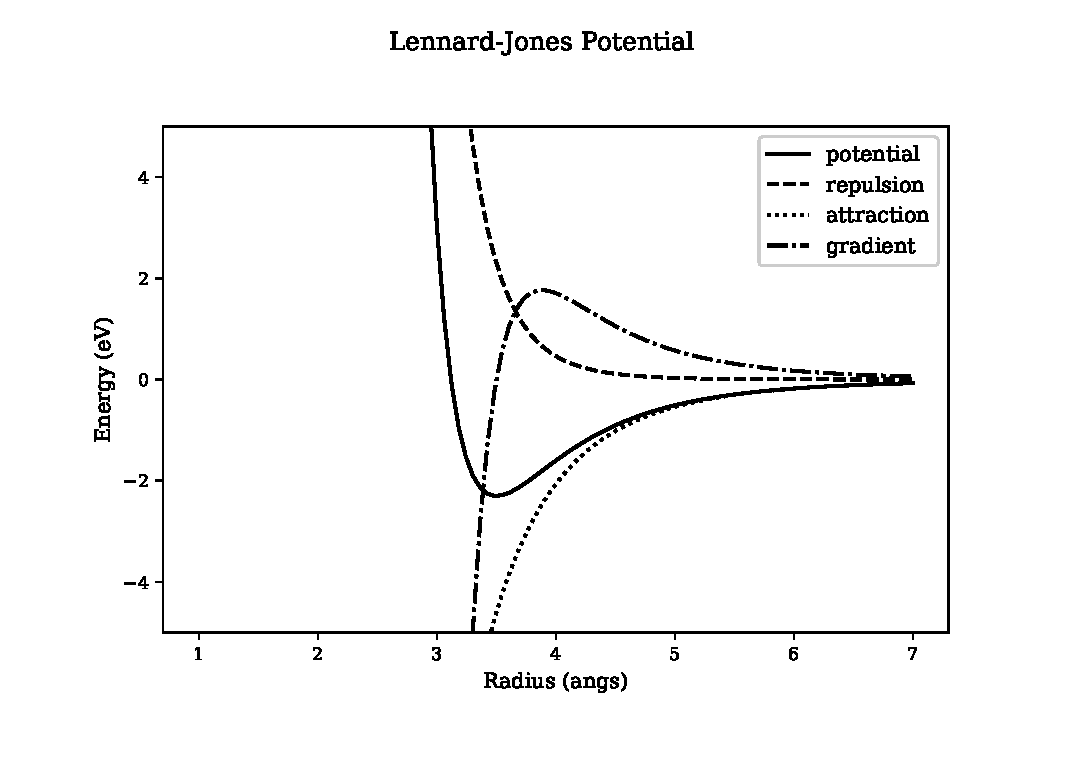
\includegraphics[width=120mm]{appendix/functions/plots/lennard_jones.eps}
    \caption{Lennard-Jones}
    \label{graph:LennardJones}
  \end{center}
\end{figure}

\begin{equation}
\begin{split}
V(r) = e \left(\left(\frac{r_m}{r}\right)^12 - 2 \left(\frac{r_m}{r}\right)^6\right)
\end{split}
\label{eq:eqLennardJones}
\end{equation}

\begin{lstlisting}[style=sPseudo,caption={Lennard-Jones potential input file}]
#A
#TYPE lennard_jones
#P 2.3 3.5
#L 0.0
#U 7.0
\end{lstlisting}

\begin{lstlisting}[style=sPseudo,caption={Lennard-Jones subroutine}]
SUBROUTINE lennard_jones(r, p, p_fixed, y)
!############################################################
! LENNARD JONES FUNCTION
IMPLICIT NONE
!############################################################
REAL(kind=DoubleReal), INTENT(IN) :: r
REAL(kind=DoubleReal), INTENT(IN) :: p(1:2)
REAL(kind=DoubleReal), INTENT(IN) :: p_fixed(1:1)
REAL(kind=DoubleReal), INTENT(OUT) :: y
!############################################################
y = p(1) * ((p(2) / r)**12 - 2 * (p(2)/r)**6)
END SUBROUTINE lennard_jones

SUBROUTINE lennard_jones_v(r, p, p_fixed, y)
!############################################################
! LENNARD JONES VECTOR FUNCTION
IMPLICIT NONE
!############################################################
REAL(kind=DoubleReal), INTENT(IN) :: r(:)
REAL(kind=DoubleReal), INTENT(IN) :: p(1:2)
REAL(kind=DoubleReal), INTENT(IN) :: p_fixed(1:1)
REAL(kind=DoubleReal), INTENT(OUT) :: y(1:SIZE(r,1))
!############################################################
INTEGER(kind=StandardInteger) :: n
!############################################################
DO n = 1, SIZE(r,1)
  CALL lennard_jones(r(n), p, p_fixed,  y(n))
END DO
END SUBROUTINE lennard_jones_v
\end{lstlisting}




\clearpage
\FloatBarrier
\subsection{Morse}

\begin{figure}[h]
  \begin{center}
    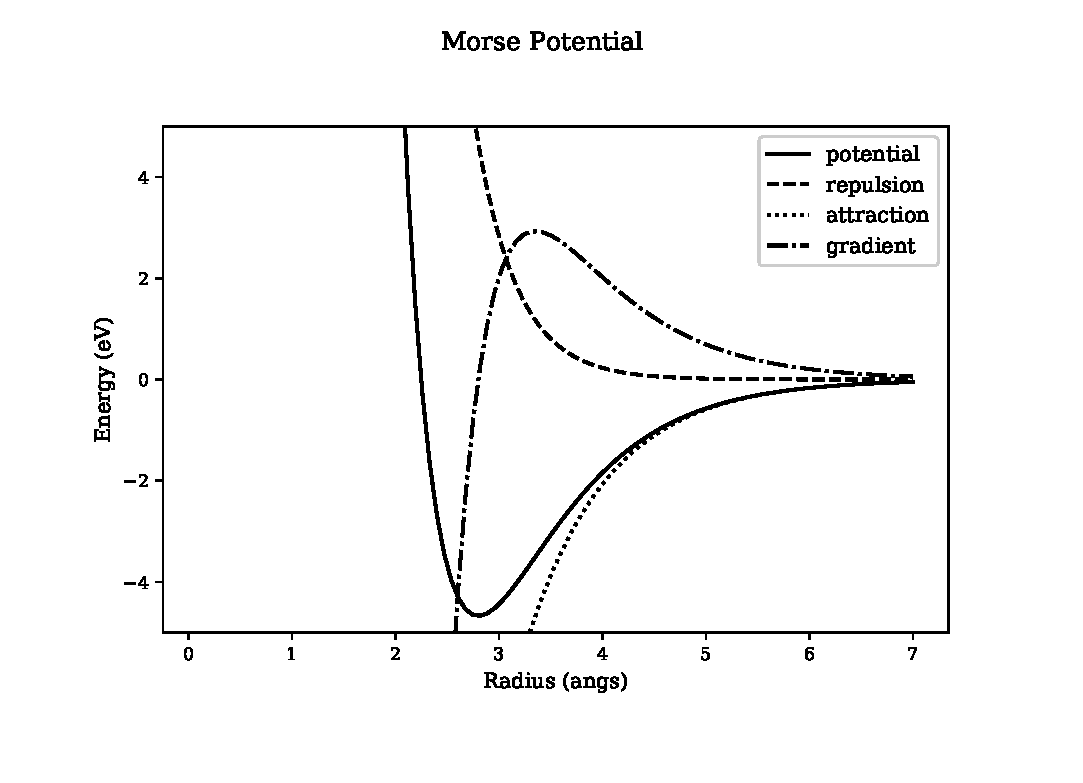
\includegraphics[width=120mm]{appendix/functions/plots/morse.eps}
    \caption{Morse}
    \label{graph:MorsePotential}
  \end{center}
\end{figure}

\begin{equation}
\begin{split}
V(r) = exp(-2 a (r - re)) - 2 exp (-a*(r - re))
\end{split}
\label{eq:eqMorse}
\end{equation}

\begin{lstlisting}[style=sPseudo,caption={Morse}]
#A
#TYPE morse
#P 4.669 1.256 2.8
#L 0.0
#U 7.0
\end{lstlisting}





\clearpage
\FloatBarrier
\subsection{Buckingham}

\begin{figure}[h]
  \begin{center}
    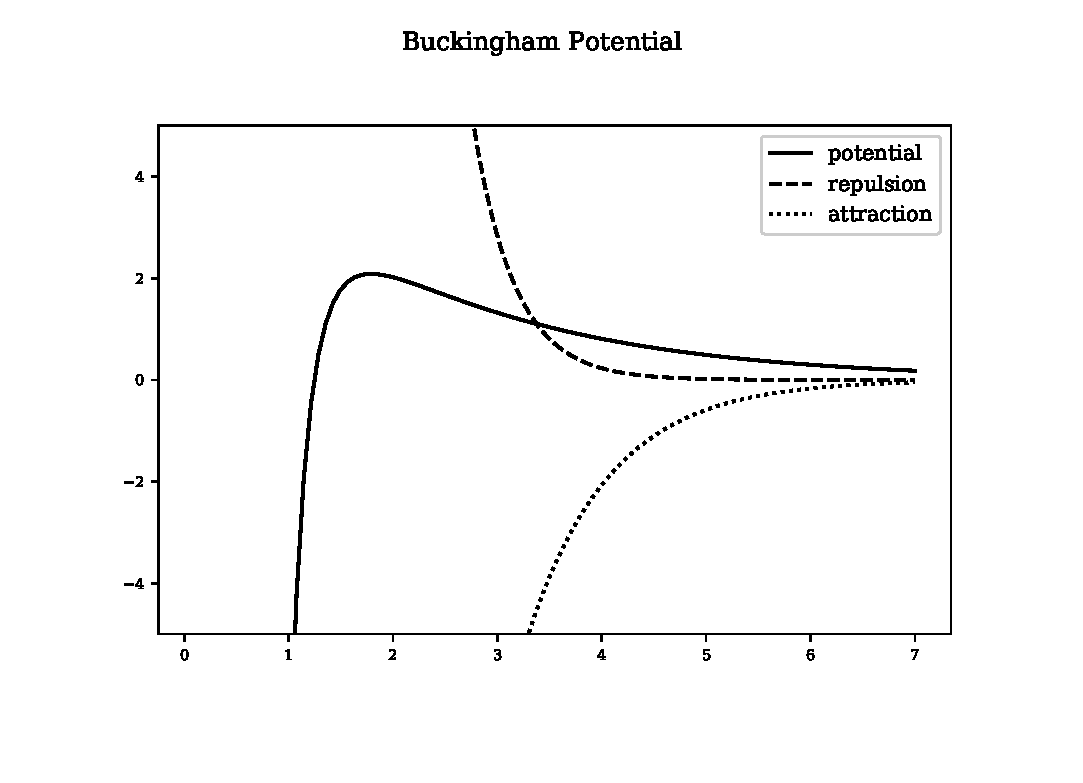
\includegraphics[width=120mm]{appendix/functions/plots/buckingham.eps}
    \caption{Buckingham}
    \label{graph:BuckinghamPotential}
  \end{center}
\end{figure}

\begin{equation}
\begin{split}
V(r) = A * exp(-B * r) - \frac{C}{r**6}
\end{split}
\label{eq:eqBuckingham}
\end{equation}

\begin{lstlisting}[style=sPseudo,caption={Buckingham}]
#A
#TYPE buckingham
#P 6.0 0.5 12.0
#L 0.0
#U 7.0
\end{lstlisting}




%\clearpage
%\FloatBarrier
%\subsection{ZBL}

%\begin{equation}
%\begin{split}
%\phi(x) = 0.181 e^{-3.2x} + 0.5099 e^{-0.9423x} + 0.2802 e^{-0.4029x} + 0.02817 e^{-0.2016x} \\
%\text{where } a_{ij} = \frac{0.8854 a_0}{Z^{0.23}_i + Z^{0.23}_j} \\
%\text{and } a_0 = 0.529 \text{angstrom}
%\end{split}
%\label{eq:screeningPotential}
%\end{equation}



%%%%%%%%%%%%%%%%%%%%%%%%%%%%%%%%%%
%       ackland_mendelev_pair    
%%%%%%%%%%%%%%%%%%%%%%%%%%%%%%%%%%


\clearpage
\FloatBarrier
\subsection{Ackland-Mendelev Pair}

%\begin{figure}[h]
%  \begin{center}
%    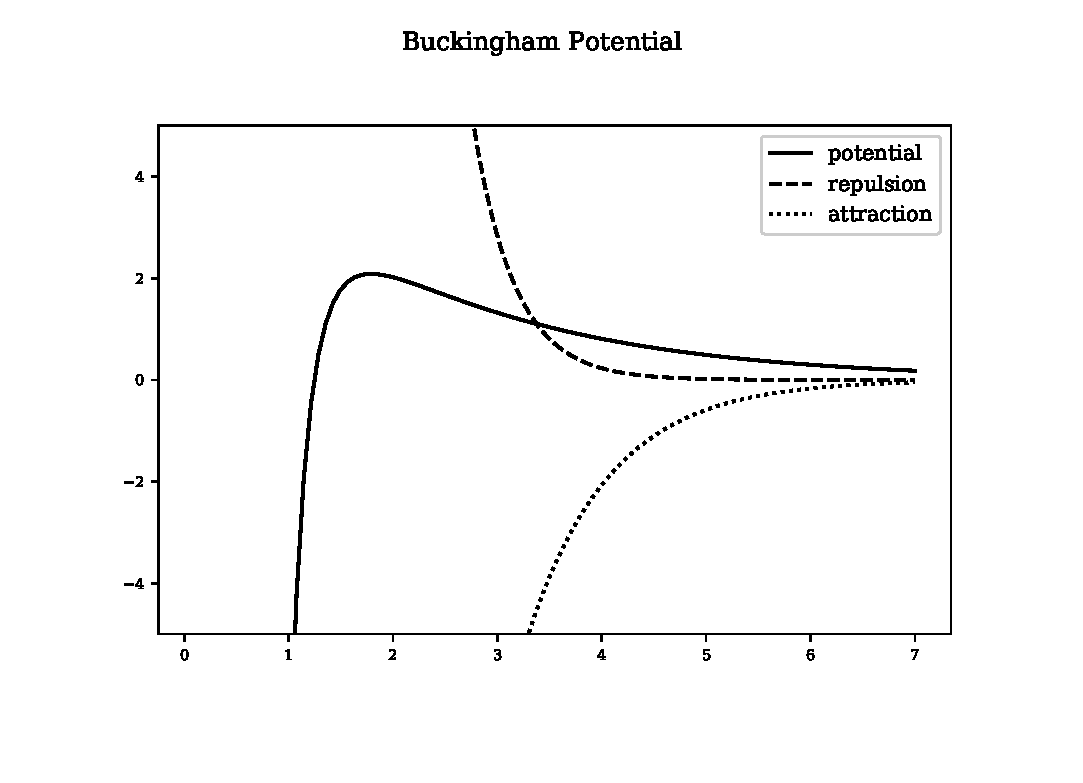
\includegraphics[width=120mm]{appendix/functions/plots/buckingham.eps}
%    \caption{Buckingham}
%    \label{graph:BuckinghamPotential}
%  \end{center}
%\end{figure}

%\begin{equation}
%\begin{split}
%V(r) = A * exp(-B * r) - \frac{C}{r**6}
%\end{split}
%\label{eq:eqBuckingham}
%\end{equation}

\begin{lstlisting}[style=sPseudo,caption={Ackland-Mendelev Pair}]
#A
#TYPE ackland_mendelev_pair
#P 6.0 0.5 12.0
#L 0.0
#U 7.0
\end{lstlisting}






%%%%%%%%%%%%%%%%%%%%%%%%%%%%%%%%%%
%       pair_spline    
%%%%%%%%%%%%%%%%%%%%%%%%%%%%%%%%%%


\clearpage
\FloatBarrier
\subsection{Pair Spline}



\begin{lstlisting}[style=sPseudo,caption={Pair Spline}]
#A
#TYPE pair_spline
#P                      0.01 -0.01  0.01  -0.01   0.01 -0.01  0.01 
#PF 26.0  26.0   1.0    1.4   2.0   3.0    4.0    4.3   5.0   5.7    6.5 
#L 0.0 
#U 7.0 
\end{lstlisting}

The first three fixed parameters specify the charge of the two species and the cutoff of the ZBL function.  The last parameter specifies where the function and its derivative goes to zero.  The pairs of variable and fixed parameters in between represent the r and v(r) values of the spline.




\clearpage
\FloatBarrier
\subsection{Quartic Polynomial Plus Exponential Repulsion}

\begin{figure}[h]
  \begin{center}
    \includegraphics[width=120mm]{appendix/functions/plots/quartic_poly_rep.eps}
    \caption{Quartic Polynomial Plus Exponential Repulsion}
    \label{graph:QuarticPolyPlusExpRep}
  \end{center}
\end{figure}

\begin{equation}
\begin{split}
H(x) = \left\{ \begin{matrix} (r - r_c)^2 (c_1 + c_1 r + c_2 r^2) + D exp(- \frac{r}{q}) & r <= r_c \\  0 & r > r_c \end{matrix} \right . 
\end{split}
\label{eq:simpleSpline}
\end{equation}

\begin{lstlisting}[style=sPseudo,caption={Quartic Polynomial with Repulsive Term}]
#A
#TYPE quartic_poly_rep
#P -4.5377 4.0659 -0.8548 9.5272e7 0.1193
#L 0.0
#U 7.0
\end{lstlisting}







\clearpage
\FloatBarrier
\section{Density Functions}

\FloatBarrier
\subsection{Quadratic Density}

\begin{figure}[h]
  \begin{center}
    \includegraphics[width=120mm]{appendix/functions/plots/quadratic_density.eps}
    \caption{Quadratic Density}
    \label{graph:QuadraticDensity}
  \end{center}
\end{figure}

\begin{equation}
\begin{split}
\rho(r) = (r - r_c)^2 
\end{split}
\label{eq:quadraticDensity}
\end{equation}

\begin{lstlisting}[style=sPseudo,caption={Quadratic Density}]
#A
#TYPE quadratic_density
#P 3.816
#L 0.0
#U 7.0
\end{lstlisting}


\clearpage
\FloatBarrier
\subsection{Slater 4S (Squared)}

\begin{figure}[h]
  \begin{center}
    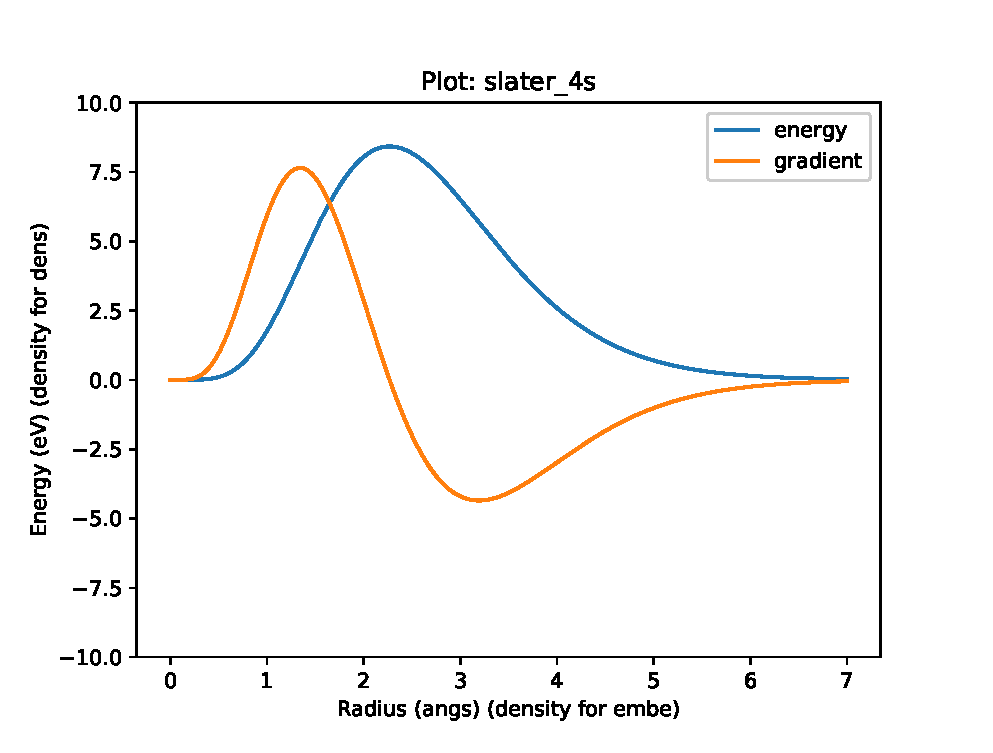
\includegraphics[width=120mm]{appendix/functions/plots/slater_4s.eps}
    \caption{Slater 4S Squared}
    \label{graph:Slater4SSquared}
  \end{center}
\end{figure}

\begin{equation}
\begin{split}
\rho(r) = (N_s r^3 exp(-\eta r))^2 
\end{split}
\label{eq:slater4S}
\end{equation}

\begin{lstlisting}[style=sPseudo,caption={Slater 4S}]
#A
#TYPE slater_4s
#P 5.0 1.323
#L 0.0
#U 7.0
\end{lstlisting}







\clearpage
\FloatBarrier
\section{Embedding Functions}

\FloatBarrier
\subsection{Finnis-Sinclair Embedding}

\begin{figure}[h]
  \begin{center}
    \includegraphics[width=120mm]{appendix/functions/plots/fs_embedding.eps}
    \caption{Finnis-Sinclair Embedding}
    \label{graph:FinnisSinclairEmb}
  \end{center}
\end{figure}

\begin{equation}
\begin{split}
F[\rho] = -A \sqrt(\rho)
\end{split}
\label{eq:fsEmbedding}
\end{equation}

\begin{lstlisting}[style=sPseudo,caption={Finnis-Sinclair Embedding}]
#A
#TYPE fs_embedding
#P 10.0
#L 0.0
#U 7.0
\end{lstlisting}



\clearpage
\FloatBarrier
\subsection{Mendelev Embedding}

\begin{figure}[h]
  \begin{center}
    \includegraphics[width=120mm]{appendix/functions/plots/mendelev_embedding.eps}
    \caption{Mendelev Embedding}
    \label{graph:MendelevEmb}
  \end{center}
\end{figure}

\begin{equation}
\begin{split}
F[\rho] = - \sqrt(\rho) + A \rho^2
\end{split}
\label{eq:mendelevEmbedding}
\end{equation}

\begin{lstlisting}[style=sPseudo,caption={Mendelev Embedding}]
#A
#TYPE mendelev_embedding
#P 10.0
#L 0.0
#U 7.0
\end{lstlisting}


\clearpage
\FloatBarrier
\subsection{Triple Embedding}

\begin{figure}[h]
  \begin{center}
    \includegraphics[width=120mm]{appendix/functions/plots/triple_embedding.eps}
    \caption{Triple Embedding}
    \label{graph:graph1}
  \end{center}
\end{figure}

\begin{equation}
\begin{split}
F[\rho] = A \sqrt(\rho) + B \rho + C \rho^2
\end{split}
\label{eq:tripleEmbedding}
\end{equation}

\begin{lstlisting}[style=sPseudo,caption={Triple Embedding}]
#A
#TYPE triple_embedding
#P -4.0 3.5 -0.1
#L 0.0
#U 7.0
\end{lstlisting}



\clearpage
\FloatBarrier
\subsection{Ackland Embedding}

\begin{figure}[h]
  \begin{center}
    \includegraphics[width=120mm]{appendix/functions/plots/ackland_embedding.eps}
    \caption{Ackland Embedding}
    \label{graph:graph1}
  \end{center}
\end{figure}

\begin{equation}
\begin{split}
F[\rho] = A \sqrt(\rho) + B \rho^2 + C \rho^4
\end{split}
\label{eq:acklandEmbedding}
\end{equation}

\begin{lstlisting}[style=sPseudo,caption={Ackland Embedding}]
#A
#TYPE ackland_embedding
#P -4.5 2.95 -0.2
#L 0.0
#U 7.0
\end{lstlisting}











\clearpage
\FloatBarrier
\section{Generic Functions}


%%%%%%%%%%%%%%%%%%%%%%%%%%%%%%%%%%
%       CUBIC SPLINE
%%%%%%%%%%%%%%%%%%%%%%%%%%%%%%%%%%

\FloatBarrier
\subsection{Cubic Spline}

\begin{figure}[h]
  \begin{center}
    \includegraphics[width=120mm]{appendix/functions/plots/cubic_spline.eps}
    \caption{Ackland Embedding}
    \label{graph:graph1}
  \end{center}
\end{figure}

\begin{equation}
\begin{split}
V(r) = \sum_i^N a_i (r - r_i)^3 H(r_i - r) \\
\text{where } \\
H(x) = \left\{ \begin{matrix} 0 & x<0 \\  1 & x >= 0 \end{matrix} \right . 
\end{split}
\label{eq:cubicSpline}
\end{equation}

This function requires two sets of parameters.  P is a list of N coefficients and PF is a list of N cutoffs.  The cubic polynomials are summed and individually scaled by the coefficients, and by virtue of its form and the heaviside step function, they cut off at the desired radius. 

\begin{lstlisting}[style=sPseudo,caption={Cubic splines potential input file}]
#A
#TYPE cubic_spline
#PF            0.976   1.150      1.216    1.650
#P          -165.0   -78.49908  -78.15495  1.8679553
#L 0.0 
#U 7.0 
\end{lstlisting}





\begin{lstlisting}[style=sPseudo,caption={Cubic splines subroutine}]
! Two Band Modelling Fe-Cr Olsson, Wallenius
! CUBIC SPLINE
! sum (ai (r - ri)^3 H(ri - r)

! SCALAR SUBROUTINE
SUBROUTINE cubic_spline(r, p, p_fixed, y)
!############################################################
! p coefficients
! pf r cutoffs
! they must be the same size
IMPLICIT NONE
!############################################################
REAL(kind=DoubleReal), INTENT(IN) :: r
REAL(kind=DoubleReal), INTENT(IN) :: p(:)
REAL(kind=DoubleReal), INTENT(IN) :: p_fixed(:)
REAL(kind=DoubleReal), INTENT(OUT) :: y
!############################################################
REAL(kind=DoubleReal) :: H
INTEGER(kind=StandardInteger) :: n
!############################################################
y = 0.0D0
DO n = 1, SIZE(p,1)
  CALL heaviside((p_fixed(n) - r), H)
  y = y + p(n) * (p_fixed(n) - r)**3 * H
END DO
IF(SIZE(p,1) + 1 .EQ. SIZE(p_fixed,1))THEN
  IF(r .GE. p_fixed(SIZE(p_fixed,1)))THEN
    y = 0.0D0
  ELSE
    y = y * ( p_fixed(SIZE(p_fixed,1) - r))**3
  END IF
END IF
END SUBROUTINE cubic_spline

! VECTOR SUBROUTINE
SUBROUTINE cubic_spline_v(r, p, p_fixed, y)
!############################################################
! CUBIC SPLINE
IMPLICIT NONE
!############################################################
REAL(kind=DoubleReal), INTENT(IN) :: r(:)
REAL(kind=DoubleReal), INTENT(IN) :: p(:)
REAL(kind=DoubleReal), INTENT(IN) :: p_fixed(:)
REAL(kind=DoubleReal), INTENT(OUT) :: y(1:SIZE(r,1))
INTEGER(kind=StandardInteger) :: n
!############################################################
! Loop through all the values in r(:), calculate and store in y(:)
DO n = 1, SIZE(r,1)
  CALL cubic_spline(r(n), p, p_fixed, y(n))
END DO
END SUBROUTINE cubic_spline_v
\end{lstlisting}





\clearpage
\FloatBarrier
\subsection{Quintic Splines}

\begin{figure}[h]
  \begin{center}
    \includegraphics[width=120mm]{appendix/functions/plots/quintic_spline.eps}
    \caption{Ackland Embedding}
    \label{graph:graph1}
  \end{center}
\end{figure}

\begin{equation}
\begin{split}
V(r) = \sum_i^N a_i (r - r_i)^5 H(r_i - r) \\
\text{where } \\
H(x) = \left\{ \begin{matrix} 0 & x<0 \\  1 & x >= 0 \end{matrix} \right . 
\end{split}
\label{eq:quinticSpline}
\end{equation}

\begin{lstlisting}[style=sPseudo,caption={Quintic Splines}]
#A
#TYPE quintic_spline
#PF 1.0 2.0  3.0 5.0 7.0
#P  0.9 2.0 -0.1 0.1 0.07
#L 0.0
#U 7.0
\end{lstlisting}






\clearpage
\FloatBarrier
\subsection{Cubic Knot Spline Fixed End}


\begin{lstlisting}[style=sPseudo,caption={Poly5 Node Spline}]
#A
#TYPE cubic_knot_spline_fixed_end
#PF  0.0  1.0  2.0  3.0    3.5   4.0   5.0   6.5   0.0   0.0   2.0
#P   0.3  0.5  0.1 -0.015  0.02  0.03  0.01
#L 0.0
#U 6.5
\end{lstlisting}







